\documentclass{article}
\usepackage[usenames]{color}
\usepackage{amsfonts}
\usepackage{amsthm}
%\usepackage{amssymb}
%\usepackage{latexsym}
%\usepackage{stmaryrd}
\usepackage{url}
\usepackage{graphicx}
\usepackage{allmtt}
\usepackage{xspace}
%\usepackage{pdfsetup}
\usepackage[a4paper,hscale=0.67,vscale=0.76]{geometry}
\usepackage{index}
\usepackage{framed}
\usepackage{boxedminipage}

\usepackage{tikzfig}
\usepackage{tikzstyles}
\usepackage{todo}

\newenvironment{graybox}
  {\def\FrameCommand{\fboxsep=0pt\colorbox{gray!20}}\MakeFramed{\smallskip\FrameRestore}\begin{quote}}
  {\end{quote}\smallskip\endMakeFramed}
\newenvironment{code}
  {\begin{graybox}\begin{allmtt}}
  {\end{allmtt}\end{graybox}}


\title{Programming Quantomatic}
\author{Lucas Dixon}

\begin{document}
\maketitle

\section{Introduction}

This is an introduction to programming Quantomatic. It is intended for
those wanting to extend the system or adapt it for some other use. For
a description of the mathematics that the system is based on,
see~\cite{2010:DDK:DCM}.

\section{Architecture}

Quantomatic consists of two programs that communicate with the each
other:

\begin{description}
\item[Quanto-Core:] is an ML program that is responsible for
  manipulating the graphs, rewrite rules and theories. It performs the
  rewriting and has a protocol for interacting with it. Quanto core
  makes use of a collection of libraries for ML called \emph{isaplib}.
\item[Quanto-Gui:] is a Java program that provide the user-interface
  for quantomatic. It starts, and then communicates with the
  Quanto-Core program.
\end{description}

Each of the programs is built on a number of libraries and contains a
number of comonents. 

\subsection{Quanto-Core}

\begin{figure}[t]
\centering{\scalebox{0.9}{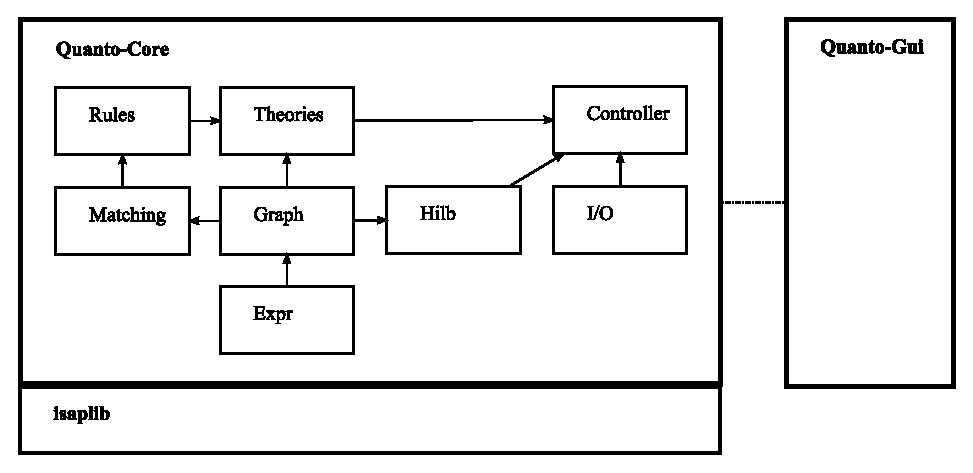
\includegraphics{arch0-core-overview}}}
\caption{The architecture of the main components of the core-part of
  quantomatic. Arrows indicate the target component using the
  source. The dotted line is the communication protocol between the
  Core component, written in ML, and the GUI one, written in Java.}
\label{fig:arch-overview1}
\end{figure}

An overview of the libraries and components, from the perspective of
the core program, is shown in Figure~\ref{fig:arch-overview1}. There
are 8 main components to the core program, all built using the common
functions provided by isaplib. These are:

\begin{description}
\item[Expression] defines a linear arithmetic expressions and
  operations on them. These expressions are used as the data stored in
  certain kinds of vertices.
\item[Graph] defines representations of graph. This provides
  structures and signatures for graphs, open graphs and bang-box
  graphs. There is a basic signature for each kinds of graph that is
  essentially only the most elementry operations needed to manipulate
  the data. The is also a signature that extends this basic
  information to provide a range of algorithms and higher-level
  functinoality.
\item[Matching] provides data structure and algorithms for matching
  graphs.
\item[Rules] defines what a graphical rewrite rule is and provides
  the functionality to applying rules to graph, using the matching
  algorithms. 
\item[Theories] are collections of rules with some meta-information,
  such as which ones should be used for automatic rewriting.
\item[I/O] provides the tools for loading and saving graphs, theories,
  expresions, etc. 
\item[Controller] defines a protocol for interacting with
  Quantomatic. This is the component that interacts with Java, and
  through which the quantomatic-core is controlled.
\item[Hilb] defines a representation of finite dimensional hilbert
  spaces using matricies. It also provides a way to interpret a
  red-green quantum graph as a such a matrix. This is used to support
  interaction with other tools, such as Mathematica.
\end{description}

An overview of the essential components for graphs, matching and
rewriting, along with the relevant components of isaplib is shown in
Figure~\ref{fig:arch-overview-in-core}.

\begin{figure}[p]
\centering{\scalebox{0.9}{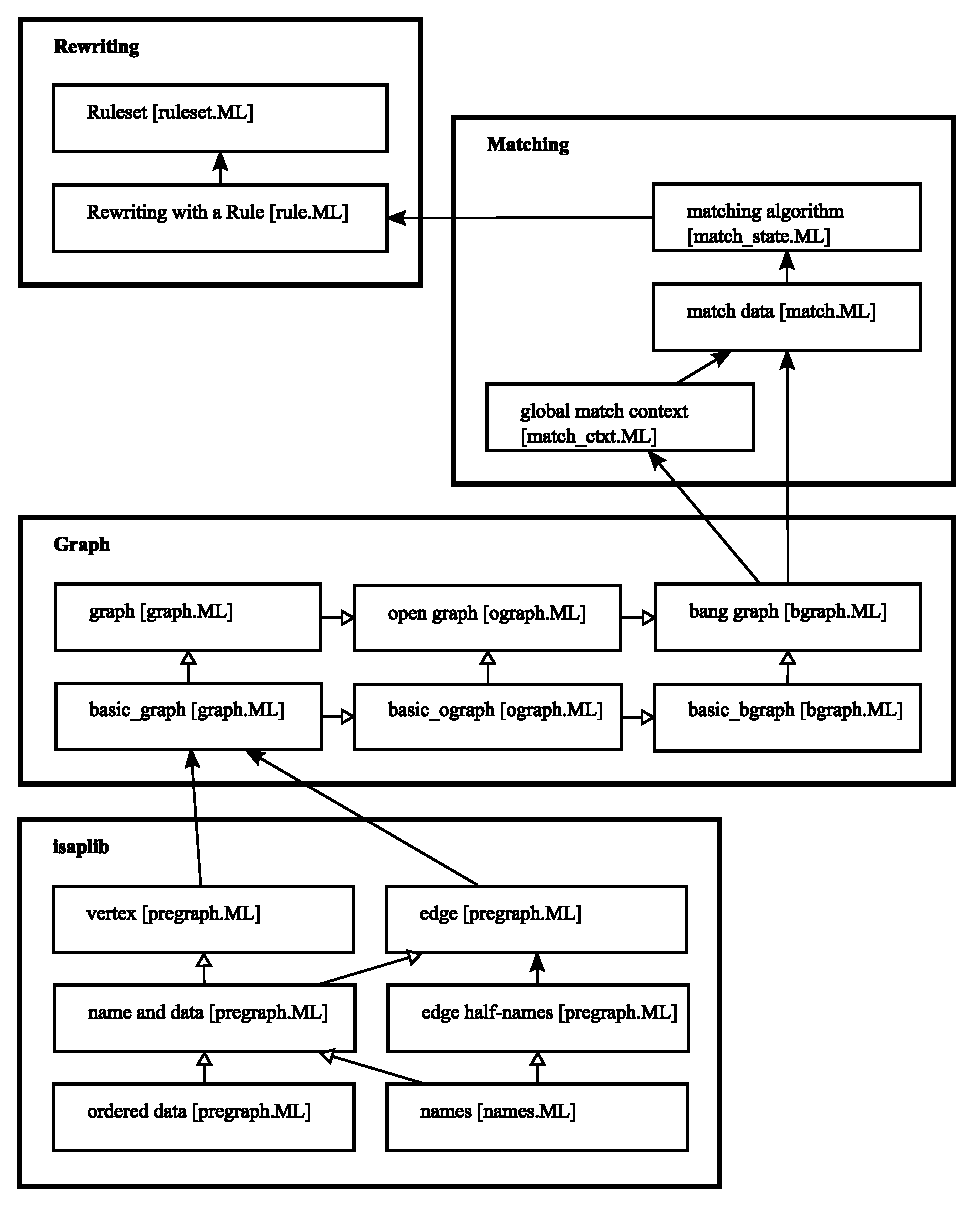
\includegraphics{arch1-names-graphs-rewriting}}}
\caption{The architecture for the construction of Graphs, Matching and
  Rewriting in Quantomatic. White-headed arrows are inheritance
  relations, and dark-headed arrows are dependency relations: the
  target uses the source.}
\label{fig:arch-overview-in-core}
\end{figure}



\subsection{Quanto-GUI}


\section{Installing, Building and Running}


\section{ML/Core}

\subsection{The SML programming language}

There is a good collection of books on programming in Standard ML including:

\begin{itemize}
\item Paulson's ``ML for the working programmer''~\cite{Paulson:ML},
  and 
\item Harper's in progress ``Programming in Standard ML'' which has a
  draft available online
  \url{http://www.cs.cmu.edu/~rwh/smlbook/online.pdf}
\end{itemize}

\subsection{PolyML}

PolyML (\url{http://www.polyml.org/}) is an efficient implementation
of Standard ML which supports efficient multi-threaded programming. 

\subsection{Editing code: jEdit and Emacs}

\begin{itemize}
\item An ML mode for emacs
  (\url{http://www.smlnj.org/doc/Emacs/sml-mode.html}), and 
\item An in-progress PolyML plugin for jEdit
  (\url{http://dream.inf.ed.ac.uk/projects/polyml/})
\end{itemize}


\subsection{Standard Basis Library}

The Standard ML Basis Library (\url{http://www.standardml.org/Basis/})
contains basic tool for interacting with the operating system.

\subsection{IsaLib Library}

{\tt isaplib/basic}: this directory contains additional libraries
beyond those of the Standard ML basis library. It builds on the
library provided by the Isabelle theorem prover. In particular, it
defines a useful collection of top-level functions and infix
operators. The most important are the following:

\begin{code}
fun I x = x

fun K x = fn \_ => x

fun x |> f = f x

fun map f [] = []
  | map f (x::xs) = (f x)::(map f xs)

fun fold f [] y = y
  | fold f (x::xs) y = fold f xs (f x y)
\end{code}

In particular, it is worth noting that the {\tt fold} function can be
understood as a more diciplined way to write a for-loop. It iterates
over all elements in a list updating the value {\tt y}, by applying
{\tt f x} to it.

\subsection{Names, name-sets, name-tables}

Rich data structures can be built up using finite sets and
mappings. For example, finite sets of names are used to identiy the
edges in a graph. A graph can then be defined as a mapping from
edge-names to the source and target vertex name. Data can be
associated to a vertex by defining a mapping from the vertex name to
the data associated with a vertex.

The key idea of name is that given a set of names, a new, fresh name
can be constructed. This allows finite sets and maps to be extended
programatically.

%% Lets use string-based names for vertices and edges. The code for this
%% is:

%% \begin{code}
%% type graph = StrNames.NTab.T 
%% \end{code}

%%  A implementation of finite
%% sets of objects

The signature that shows most of the functions for working with finite
sets of names can be found in: \begin{center}{\tt
  isaplib/names/basic\_nameset.ML}\end{center}

Map from a finite set of names to some other type are called
name-tables and the signature showing most of the functions for
working with them can be found in: \begin{center}{\tt
  isaplib/names/basic\_nametab.ML}\end{center}


\subsection{Renaming}



\subsection{Maps, Isomorphisms and Binary Relations}



\subsection{Graphs}


\subsection{Matching}


\subsection{I/O}


\subsection{Controller}



\bibliographystyle{plain}
\bibliography{bibfile}


\end{document}
